Cells can be simply described as an insulating lipid bilayer with voltage controlled ion channels. As such, they can be described simply via equivalent circuit models, the simplest of such is modelling the membrane as a capacitor and the ion channels as resistors (see figure \ref{fig3.1}). To electronically model action potentials however, a more complex circuit is needed as ion channels do not behave as linear resistors. Instead a channel is modelled as a non-linear current voltage device. \par

The Bonhoeffer-Van der Pol (BVP) electronic model of a single cell action potential is one of the simplest ways to achieve this. In the BVP model the non-linear current voltage device is created by a series voltage source and diode in parallel to an inductor and resistor (see appendix \ref{appendixVDP}). The BVP model was expanded in the original development of the FN model to simulate a nerve axon \citep{fitzhughnagumo}. This was achieved by coupling BVP circuits in a linear fashion as discussed in appendix \ref{appendixVDP}. \par 

A modern simple alternative to the non-linear current voltage devices is to use transistors to control the gating of the simulated ion channels. One circuit that can be accurately described by a FN equation is a three transistor model described by Lancaster and Hellen \citep{3transistor}. This model (shown in figure \ref{fig3.4}) simulates a self exciting cell action potential which has a very similar membrane potential output as predicted by FN equations, where the capacitor voltage represents the membrane potential and the transistor base voltage is the inhibitory variable. \par

\begin{figure}[H]
    \centering
    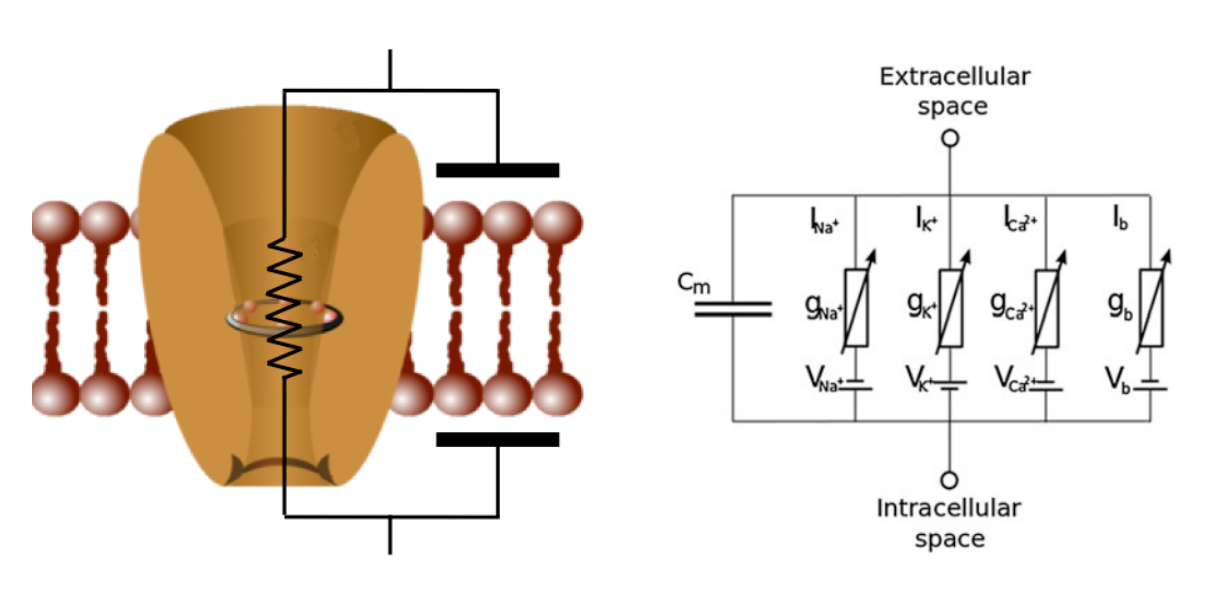
\includegraphics[width=0.8\textwidth]{images/simpleelectronic.png}
    \caption{Left: A simple equivalent circuit model for a cell membrane and ion channel. The system can be represented as a parallel RC circuit \citep{simpleelectronic}. Right: The RC model applied to a cardiac cell where the major ion channels of interest are included. Voltage variable resistors are used to act as the voltage gated ion channels. \citep{phdpaper}}
    \label{fig3.1}
\end{figure}

\begin{SCfigure}[0.9][h!]
    \centering
    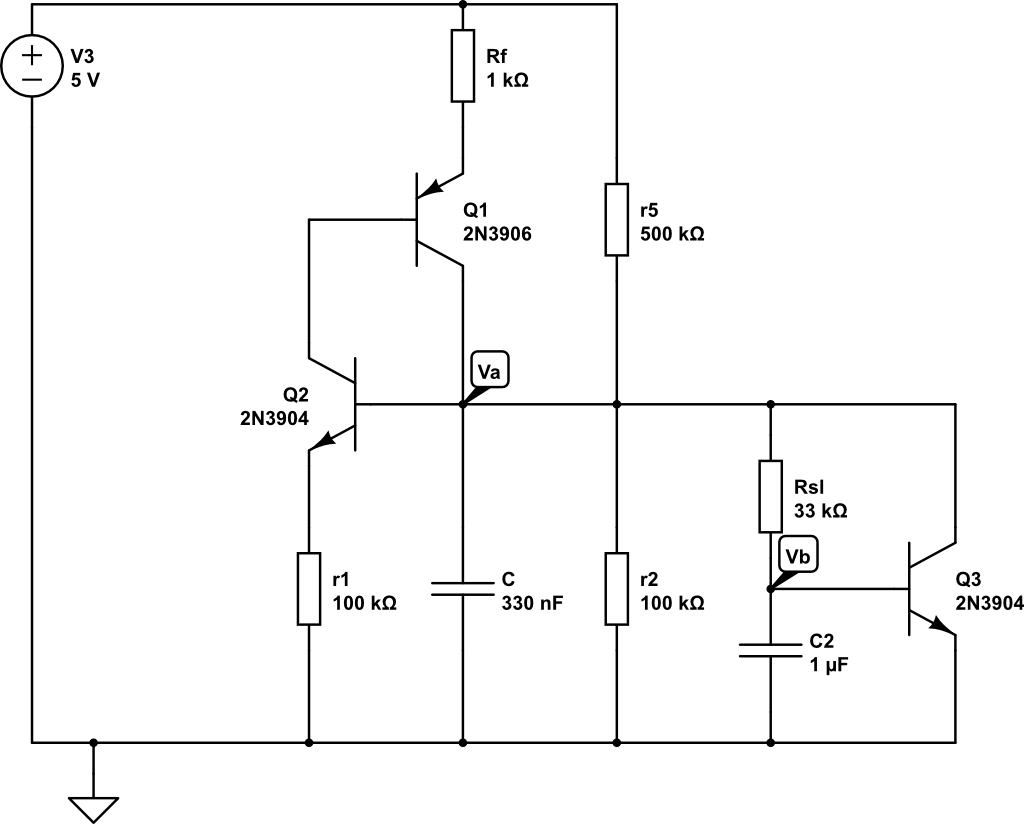
\includegraphics[width=0.5\textwidth]{images/3-transistor-circuit.png}
    \caption{A circuit diagram of the 3 transistor cell model with components identified. $V_a$ is the membrane potential and $V_b$ the inhibitory variable. The two left hand transistors are responsible for the fast-response positive feedback required for the depolarisation phase. The final transistor is responsible for the inhibitory variable.}
    \label{fig3.4}
\end{SCfigure}

\subsection{Electronic Model of an Isolated Cell}
Using the three transistor circuit shown in figure \ref{fig3.4} we computationally simulated the circuits output. The circuit shows a self exciting action potential which can be used to simulate a single excitable cell.
\begin{figure}[H]
    \centering
    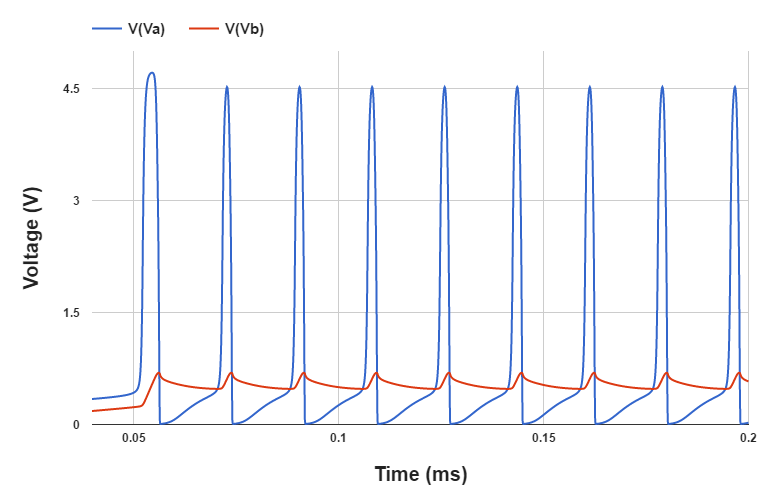
\includegraphics[width=0.7\textwidth]{images/singlecellelec.png}
    \caption{The simulated output of voltmeters placed at positions $V_a$ (the membrane potential) and $V_b$ (the inhibitory variable) shown in figure \ref{fig3.4}.}
    \label{fig3.5}
\end{figure}

\subsection{2D Electronic Model}
By combining these individual 'cells' together in a ring, we can simulate a 2D 'slice' of the atrium. We first simulated this circuit computationally and then created the physical circuit to measure via an oscilloscope, a photo of the full circuit and a full circuit diagram can be seen in appendix \ref{appendixcircuit}. 6 individual cells were used in a ring with the first cell acting as the SAN and each neighbouring cell receiving the output of the previous cell via a resistor (which acts as the extra-cellular diffusion time) as its stimulation current. The final cell receives two inputs simultaneously exciting it. The final cells excitation does not propagate back round as each of its neighbours are in a relaxation state and unable to be excited again, this terminates the current. A regular pulse is observed.
\begin{figure}[H]
    \centering
    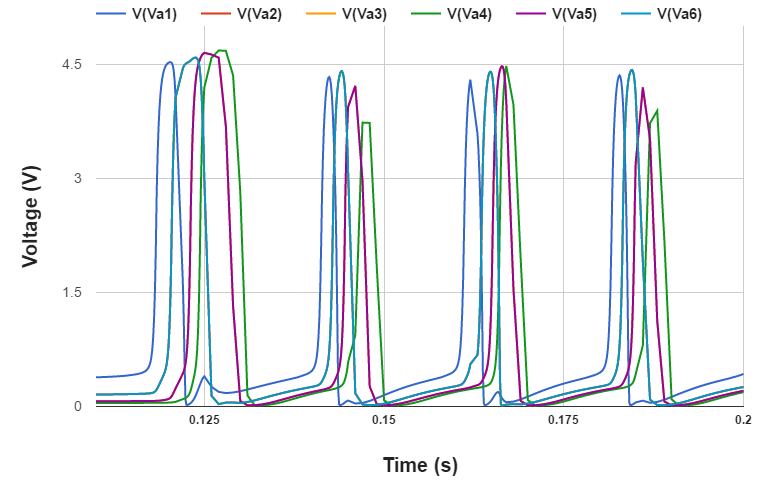
\includegraphics[width=0.7\textwidth]{images/6cellnoblock.png}
    \caption{The simulated output of voltmeters placed at positions $V_a$ (the membrane potential) in figure \ref{fig3.4} for cells 1 though 6 in the ring network shown in appendix \ref{appendixcircuit}.}
    \label{fig3.7}
\end{figure}


\subsection{Simulation of Re-entrant Tachycardia}
As shown in the 2D 6 cell circuit diagram shown in appendix \ref{appendixcircuit}, two switches and a diode can be added between each cell. The switch parallel to the diode can be opened to create a uni-directional blocker and thus simulate tachycardia. The blocker stops current flowing in the forward direction. \par

As an example, opening the switch between cells 6 and 5 (numbering clockwise) means cell 4 does not excite via the forward propagation. Instead, it remains relaxed allowing the AVN cell (cell 3) to excite it. In turn cell 5 has relaxed by this point allowing it to re-excite. This causes an increase in the pulse rate of the circuit as shown in figure \ref{fig3.8}. \par
\begin{figure}[H]
    \centering
    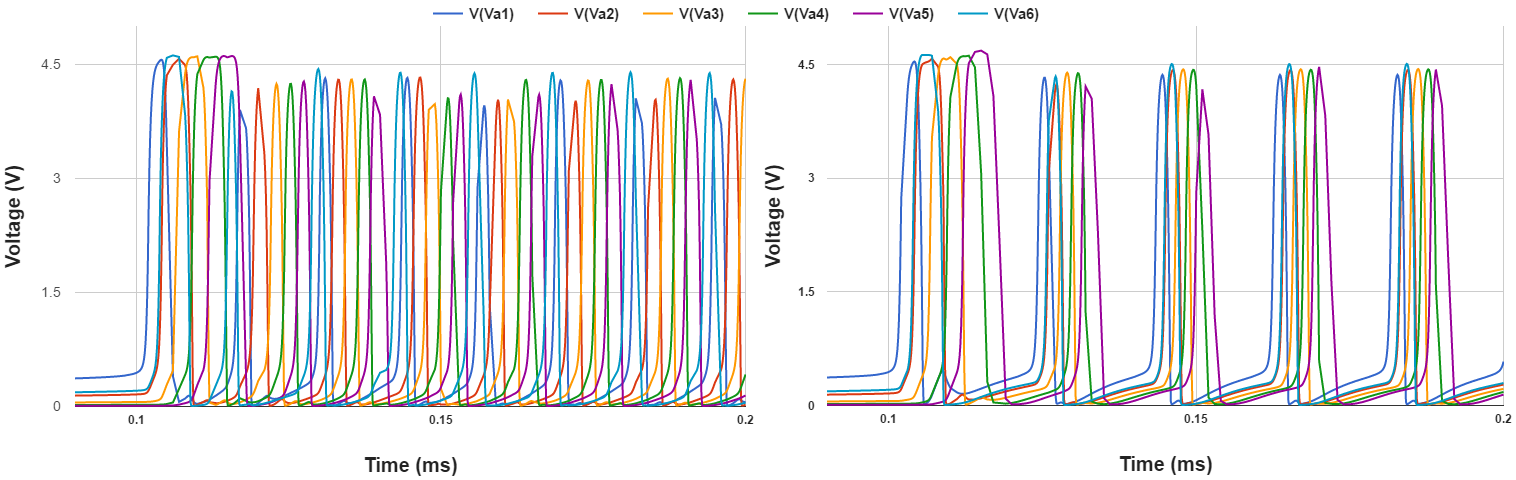
\includegraphics[width=\textwidth]{images/Electronic6cell.png}
    \caption{Left: The simulated output of voltmeters placed at positions $V_a$ (the membrane potential) in figure \ref{fig3.4} for cells 1 through 6 in figure \ref{fig3.6} in the presence of a uni-directional blocker between cells 6 and 5. Right: The same output for cells 1 through 6 in the presence of an omni-directional blocker between cells 6 and 5.}
    \label{fig3.8}
\end{figure}

One treatment for re-entrant tachycardia is ablation. This is where the uni-directional blocker is destroyed via the surgical placement of catheters and radio-frequency irradiation. The destruction of the abnormal cells transforms the uni-directional blocker into an omni-directional blocker. In the circuit model this is achieved by opening the series switch between cells 6 and 5. This stops the re-entrant current, curing the tachycardia and returning the pulse rate to normal, as shown in figure \ref{fig3.8}. 

\subsection{Further Development of the Electronic Model}
The three transistor electronic model described above is clearly limited in complexity and scale. The action potential is also not an accurate simulation of a cardiac action potential as it lacks a calcium ion controlled plateau phase. The model, in theory, could be expanded into a cubic 3D lattice or even hollow spherical structure to better simulate the heart's geometry. However, the model would start to suffer anisotropy issues as the cell circuits are designed in a linear arrangement. \par

The linear limitations of the model, as well as the action potential shape, better suit it for use in modelling nerve axon potentials. Manipulating the circuit to create an action potential more reminiscent of a cardiac action potential will require different components. Due to the limitations of using generic electrical components, this involves redesigning the circuit for every parameter change. As such we terminated development of the model here and pursued a computational path.